\documentclass{article}
\usepackage[utf8]{inputenc}

\usepackage{enumitem}
\usepackage{hyperref}
\usepackage{graphicx}
\usepackage{float}

\hypersetup{
    colorlinks=true,
    urlcolor=blue,
}

\title{TDT4305: Project Phase 1\\Exploratory Analysis of Twitter Dataset}
\author{Fredrik Bakken and Tor Arne Hagen}
\date{\today}

\begin{document}

\maketitle

\newpage

% QUESTION 1
\section*{Task 1: Load RDD and Explore}
\subsection*{Source Code and Results}
    \begin{itemize}
        \item \textbf{Source code:} task\_1.py (\href{https://github.com/FredrikBakken/TDT4305_Big-Data-Project/blob/master/PhaseOne/task_1.py}{Github})
        \item \textbf{Results:} /data/results/result\_1.tsv (\href{https://github.com/FredrikBakken/TDT4305_Big-Data-Project/blob/master/PhaseOne/data/results/result_1.tsv}{Github})
    \end{itemize}

\subsection*{Questions to be Answered}
\begin{enumerate}[label=\alph*)]
    % Question 1a
    \item \textit{How many tweets are there?}\\
    
    Total number of tweets: \textbf{2715066}.\\
    
    Solved by using the Spark function \textit{.count()} on the entire RDD data set.\\ \\
    
    
    % Question 1b
    \item \textit{How many distinct users (username) are there?}\\
    
    Number of distinct usernames: \textbf{499822}.\\
    
    Solved by using the Spark functions \textit{.map()}, \textit{.distinct()}, and \textit{.count()} on the USERNAME row of the data set.\\ \\
    
    
    % Question 1c
    \item \textit{How many distinct countries (country\_name) are there?}\\
    
    Number of distinct country names: \textbf{70}.\\
    
    Solved by using the Spark functions \textit{.map()}, \textit{.distinct()}, and \textit{.count()} on the COUNTRY\_NAME row of the data set.\\ \\
    
    
    % Question 1d
    \item \textit{How many distinct places (place\_name) are there?}\\
    
    Number of distinct place names: \textbf{23121}.\\
    
    Solved by using the Spark functions \textit{.map()}, \textit{.distinct()}, and \textit{.count()} on the PLACE\_NAME row of the data set.\\ \\
    
    
    % Question 1e
    \item \textit{In how many languages users post tweets?}\\
    
    Number of distinct languages: \textbf{46}.\\
    
    Solved by using the Spark functions \textit{.map()}, \textit{.distinct()}, and \textit{.count()} on the LANGUAGE row of the data set.\\ \\
    
    
    % Question 1f
    \item \textit{What is the minimum latitude?}\\
    
    Minimum latitude: \textbf{-54.87555556}.\\
    
    Solved by using the Spark function \textit{.min()} on the LATITUDE row of the data set.\\ \\
    
    
    % Question 1g
    \item \textit{What is the minimum longitude?}\\
    
    Minimum longitude: \textbf{-159.83019441}.\\
    
    Solved by using the Spark function \textit{.min()} on the LONGITUDE row of the data set.\\ \\
    
    
    % Question 1h
    \item \textit{What is the maximum latitude?}\\
    
    Maximum latitude: \textbf{69.83186826}.\\
    
    Solved by using the Spark function \textit{.max()} on the LATITUDE row of the data set.\\ \\
    
    
    % Question 1i
    \item \textit{What is the maximum longitude?}\\
    
    Maximum longitude: \textbf{153.03508445}.\\
    
    Solved by using the Spark function \textit{.max()} on the LONGITUDE row of the data set.\\ \\
    
    
    % Question 1j
    \item \textit{ What is the average length of a tweet text in terms of characters?}\\
    
    Average number of characters in each tweet: \textbf{87.2014098368}.\\
    
    Solved by using the Spark functions \textit{.map()} and \textit{.mean()} on the length of the TWEET\_TEXT row of the data set.\\ \\
    
    
    % Question 1k
    \item \textit{What is the average length of a tweet text in terms of words?}\\
    
    Average number of words in each tweet: \textbf{12.2284228081}.\\
    
    Solved by using the Spark functions \textit{.map()} and \textit{.mean()} on the split (by empty space) length of the TWEET\_TEXT row of the data set.\\ \\
\end{enumerate}


% QUESTION 2
\section*{Task 2: Tweet Counts per Country}
\subsection*{Source Code and Results}
    \begin{itemize}
        \item \textbf{Source code:} task\_2.py (\href{https://github.com/FredrikBakken/TDT4305_Big-Data-Project/blob/master/PhaseOne/task_2.py}{Github})
        \item \textbf{Results:} /data/results/result\_2.tsv (\href{https://github.com/FredrikBakken/TDT4305_Big-Data-Project/blob/master/PhaseOne/data/results/result_2.tsv}{Github})
    \end{itemize}

\subsection*{Questions to be Answered}
\begin{enumerate}[label=\alph*)]
    \item \textit{Find the total number of tweets posted from each country and sort them in descending order of tweet counts. For countries with equal number of tweets, sorting must be in alphabetical order.}\\
    
    ANSWER...\\ \\
\end{enumerate}


% QUESTION 3
\section*{Task 3: Geographical Centroids per Country}
\subsection*{Source Code and Results}
    \begin{itemize}
        \item \textbf{Source code:} task\_3.py (\href{https://github.com/FredrikBakken/TDT4305_Big-Data-Project/blob/master/PhaseOne/task_3.py}{Github})
        \item \textbf{Results:} /data/results/result\_3.tsv (\href{https://github.com/FredrikBakken/TDT4305_Big-Data-Project/blob/master/PhaseOne/data/results/result_3.tsv}{Github})
    \end{itemize}

\subsection*{Questions to be Answered}
\begin{enumerate}[label=\alph*)]
    \item \textit{Write a code (named "task\_3") that outputs in a TSV file the latitude and longitude of the centroids and the names of the countries, in the form of \textless country\_name\textgreater tab\textless latitude\textgreater tab\textless longitude\textgreater .}\\
    
    The final code solution in task 3 uses a method which creates an extreme run-time of more 30min. Eventhough the execution time is extremely slow because of so many Spark tasks, it still gives the correct result.\\
    
    A more efficient solution would take advantage of the aggregation method.\\
    
    \item \textit{Visualize the results in CartoDB.}\\
    
    \begin{figure}[H]
        \centering
        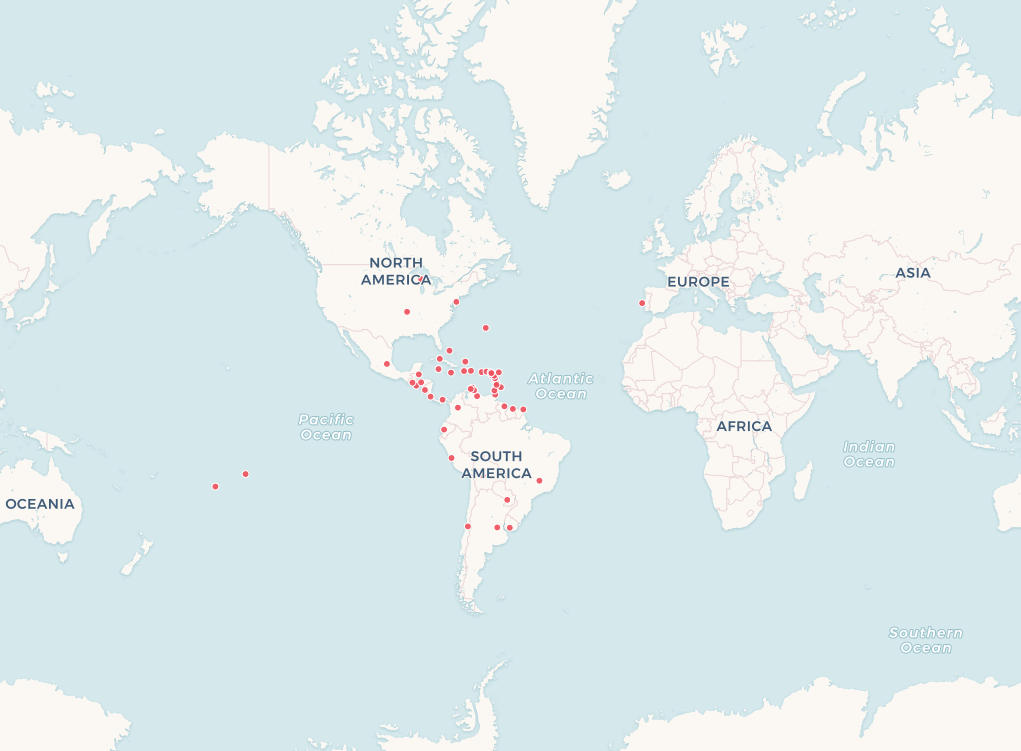
\includegraphics[width=\textwidth]{PhaseOne/docs/img/cartodb-visualization.png}
        \caption{Result Visualization in CartoDB.}
        \label{fig:cartodb}
    \end{figure}
    
\end{enumerate}


% QUESTION 4
\section*{Task 4: Most Active Hours per Country}
\subsection*{Source Code and Results}
    \begin{itemize}
        \item \textbf{Source code:} task\_4.py (\href{https://github.com/FredrikBakken/TDT4305_Big-Data-Project/blob/master/PhaseOne/task_4.py}{Github})
        \item \textbf{Results:} /data/results/result\_4.tsv (\href{https://github.com/FredrikBakken/TDT4305_Big-Data-Project/blob/master/PhaseOne/data/results/result_4.tsv}{Github})
    \end{itemize}

\subsection*{Questions to be Answered}
\begin{enumerate}[label=\alph*)]
    \item \textit{Question...}\\
    
    ANSWER...\\ \\
\end{enumerate}


\section*{Task 5: Tweet Counts per City}
\subsection*{Source Code and Results}
    \begin{itemize}
        \item \textbf{Source code:} task\_5.py (\href{https://github.com/FredrikBakken/TDT4305_Big-Data-Project/blob/master/PhaseOne/task_5.py}{Github})
        \item \textbf{Results:} /data/results/result\_5.tsv (\href{https://github.com/FredrikBakken/TDT4305_Big-Data-Project/blob/master/PhaseOne/data/results/result_5.tsv}{Github})
    \end{itemize}

\subsection*{Questions to be Answered}
\begin{enumerate}[label=\alph*)]
    \item \textit{Question...}\\
    
    ANSWER...\\ \\
\end{enumerate}

\section*{Task 6: Frequent Words in a Country}
\subsection*{Source Code and Results}
    \begin{itemize}
        \item \textbf{Source code:} task\_6.py (\href{https://github.com/FredrikBakken/TDT4305_Big-Data-Project/blob/master/PhaseOne/task_6.py}{Github})
        \item \textbf{Results:} /data/results/result\_6.tsv (\href{https://github.com/FredrikBakken/TDT4305_Big-Data-Project/blob/master/PhaseOne/data/results/result_6.tsv}{Github})
    \end{itemize}

\subsection*{Questions to be Answered}
\begin{enumerate}[label=\alph*)]
    \item \textit{Question...}\\
    
    ANSWER...\\ \\
\end{enumerate}

\section*{Task 7: Frequent Words per City}
\subsection*{Source Code and Results}
    \begin{itemize}
        \item \textbf{Source code:} task\_7.py (\href{https://github.com/FredrikBakken/TDT4305_Big-Data-Project/blob/master/PhaseOne/task_7.py}{Github})
        \item \textbf{Results:} /data/results/result\_7.tsv (\href{https://github.com/FredrikBakken/TDT4305_Big-Data-Project/blob/master/PhaseOne/data/results/result_7.tsv}{Github})
    \end{itemize}

\subsection*{Questions to be Answered}
\begin{enumerate}[label=\alph*)]
    \item \textit{Question...}\\
    
    ANSWER...\\ \\
\end{enumerate}

\section*{Task 8: Explore using Spark SQL and Dataset API}
\subsection*{Source Code and Results}
    \begin{itemize}
        \item \textbf{Source code:} task\_8.py (\href{https://github.com/FredrikBakken/TDT4305_Big-Data-Project/blob/master/PhaseOne/task_8.py}{Github})
        \item \textbf{Results:} /data/results/result\_8.tsv (\href{https://github.com/FredrikBakken/TDT4305_Big-Data-Project/blob/master/PhaseOne/data/results/result_8.tsv}{Github})
    \end{itemize}

\subsection*{Questions to be Answered}
\begin{enumerate}[label=\alph*)]
    \item \textit{Question...}\\
    
    ANSWER...\\ \\
\end{enumerate}

\end{document}